% https://www.zhihu.com/question/1890528932589195405/answer/1922318598199842050
\documentclass[tikz,border=1cm]{standalone}
\usetikzlibrary{shapes.geometric}
\usetikzlibrary{positioning}
\usetikzlibrary{decorations.markings}
% https://tex.stackexchange.com/questions/96967/how-can-i-strike-out-arrows-in-tikz
\newcommand*{\StrikeThruDistance}{.1cm}%
\newcommand*{\StrikeThru}{\StrikeThruDistance,\StrikeThruDistance}%
\tikzset{strike thru arrow/.style={
    decoration={markings, mark=at position 0.5 with {
        \draw [black,-] 
            ++ (-\StrikeThruDistance,-\StrikeThruDistance) 
            -- ( \StrikeThruDistance, \StrikeThruDistance);}
    },
    postaction={decorate},
}}
\tikzset{
    trapezium stretches = true,
    mynodea/.style={
        draw,trapezium,text=black,
        shape border rotate=270,
        fill=#1!20,draw=#1!75,
        minimum height=.8cm,
        outer sep=0pt,
        inner sep=1pt,
        },
    mynodeb/.style={
        dashed,diamond,text=black,
        shape border rotate=270,
        fill=#1!20,draw=#1!75,
        minimum size=.8cm,
        inner sep=0pt,
        outer sep=0pt,
        },
    plainnode/.style={
        rectangle,minimum size=.5cm,
        outer sep=0pt,inner sep=1pt,
        }
    }
\begin{document}

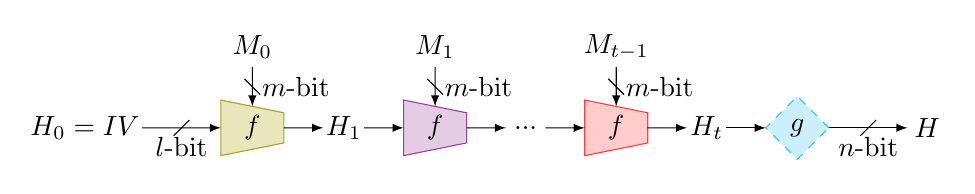
\begin{tikzpicture}
    \node[plainnode] (H) {$H$};
    \node[mynodeb=cyan] (G) [left=of H] {$g$} edge [-latex,strike thru arrow] node[auto,swap] {$n$-bit} (H);
    \node[plainnode] (Ht) [left=.5cm of G] {$H_t$} edge[-latex] (G);
    \node[mynodea=red] (f3) [left=.5cm of Ht] {$f$} edge[-latex] (Ht);
    \node[plainnode] (ell) [left=.5cm of f3] {...} edge[-latex] (f3);
    \node[mynodea=violet] (f2) [left=.5cm of ell] {$f$} edge[-latex] (ell);
    \node[plainnode] (H1) [left=.5cm of f2] {$H_1$} edge[-latex] (f2);
    \node[mynodea=olive] (f1) [left=.5cm of H1] {$f$} edge[-latex] (H1);
    \node[plainnode] (H0) [left=of f1] {$H_0=IV$} edge[-latex,strike thru arrow] node[auto,swap] {$l$-bit} (f1);
    \node[plainnode,inner sep=0pt] (Mt-1) [above=.5cm of f3] {$M_{t-1}$} edge [-latex,strike thru arrow] node[auto] {$m$-bit} (f3);
    \node[plainnode,inner sep=0pt] (M1) [above=.5cm of f2] {$M_1$} edge [-latex,strike thru arrow] node[auto] {$m$-bit} (f2);
    \node[plainnode,inner sep=0pt] (M0) [above=.5cm of f1] {$M_0$} edge [-latex,strike thru arrow] node[auto] {$m$-bit} (f1);
\end{tikzpicture}
\end{document}